\section{3D walking}

In the frame of the \koroibot\ project we had to make the robot going through stair cases and stepping stones.
Moreover partners from Airbus asked if it was feasible to walk and climb stairs with an industrial tool in the robot hand.
Hence the goal of this fourth behavior was to design a walking pattern generator able to make HRP-2 climbing and going down stairs with a tool in the gripper.

\begin{figure}[ht]
  \begin{center}
    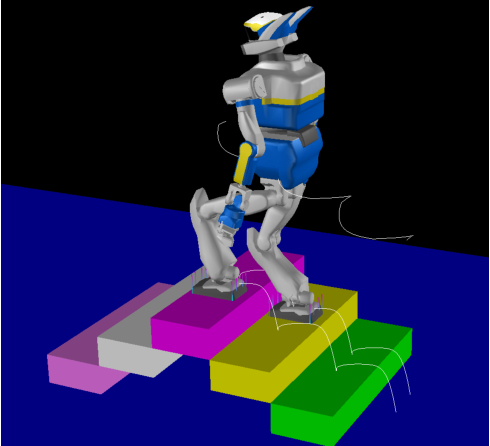
\includegraphics[clip=true, keepaspectratio, height=0.28\linewidth]
    {./figures/PastedGraphic-2.pdf}\\[0.05cm]
    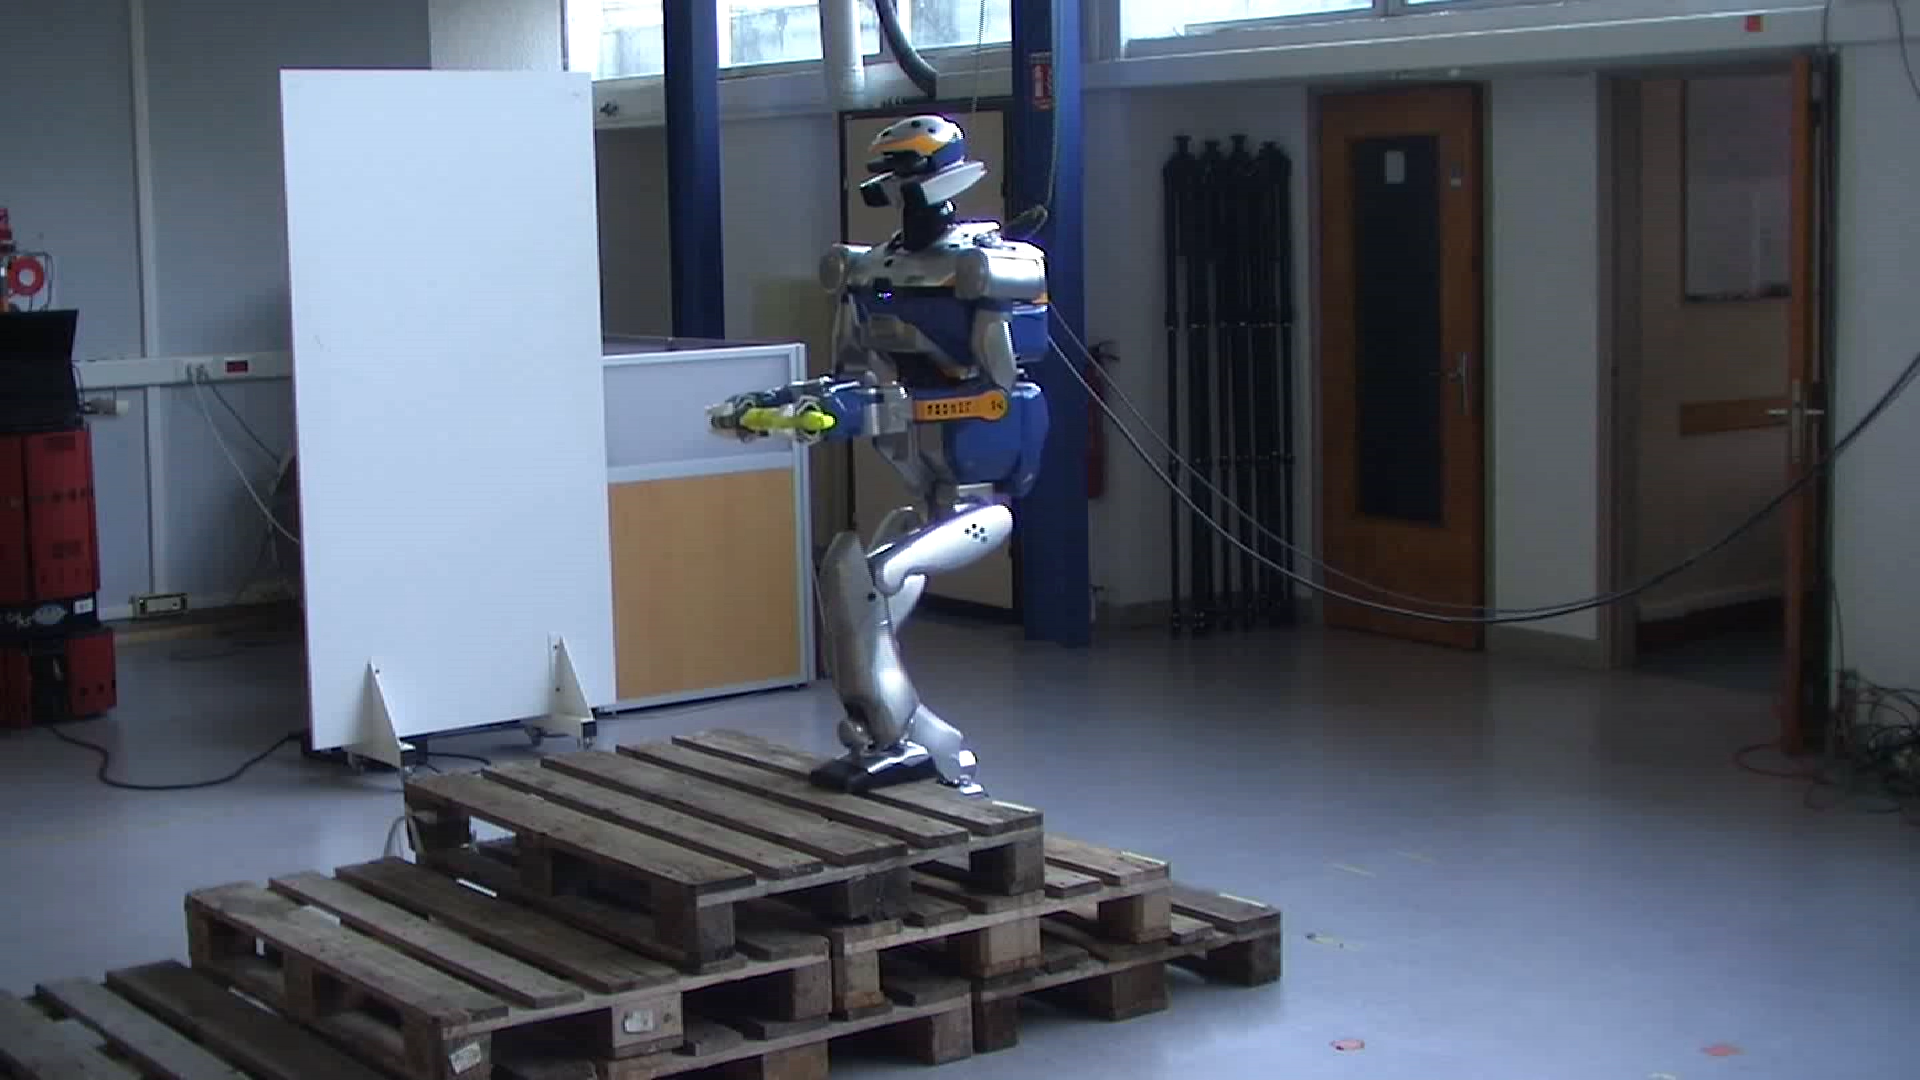
\includegraphics[clip=true, keepaspectratio, height=0.28\linewidth]
    {./figures/goinguptoolpalette.png}\hfill
    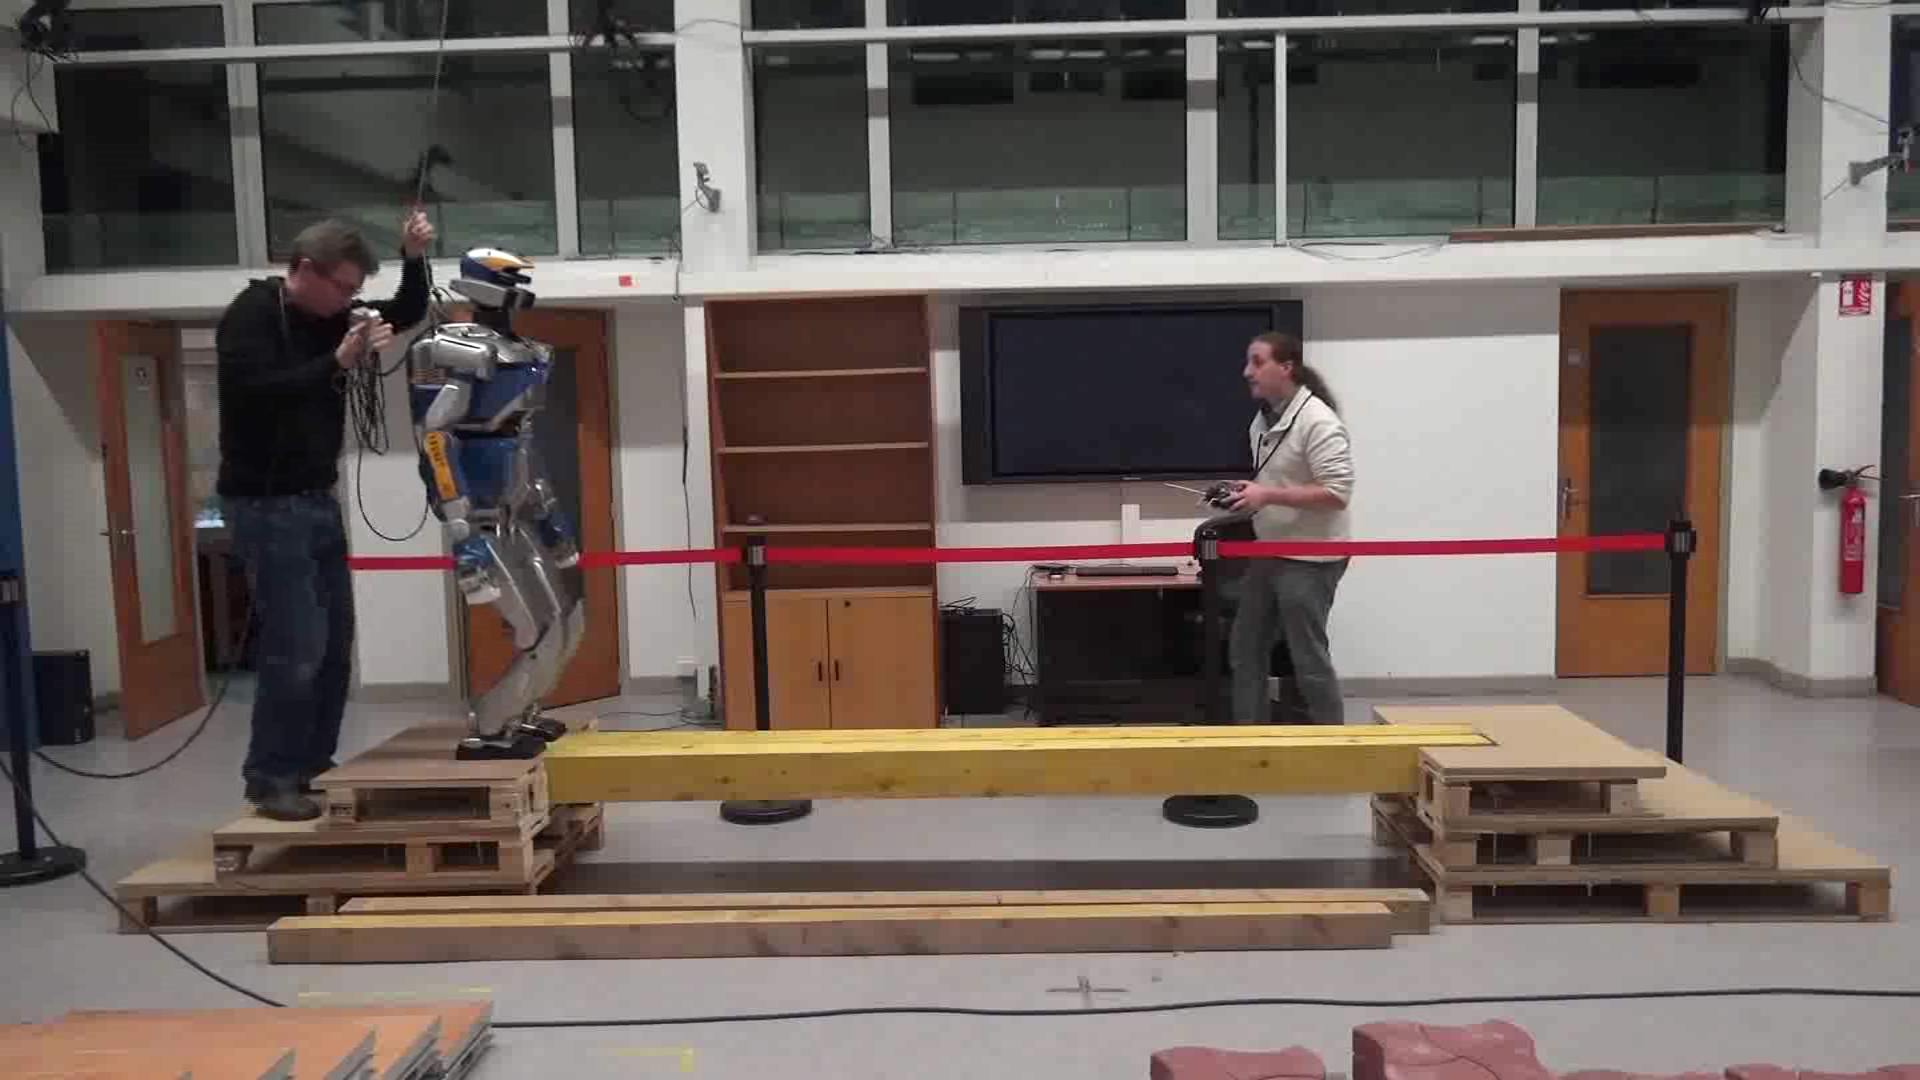
\includegraphics[clip=true, keepaspectratio, height=0.28\linewidth]
    {./figures/beam.png}   
  \end{center}
  \caption{The first two images depicts HRP-2 climbing stair in the 3D environment of OpenHRP and on the real stairs. The last one show HRP-2 ready to walk on a beam.
  }
  \label{fig:old:stairs}
\end{figure}

At the beginning of my thesis their were no controller in LAAS-CNRS able to make HRP-2 
going though stair cases.
Two developments had to be made.
First the development of need 3D trajectories for the feet.
And second the development of new 3D CoM trajectories.
We decided to use the existing walking pattern generator from \cite{stasse2009fast} and extend it to 3D walking.
The results are presented in \cite{naveau:ichr:2014}.
The video of the motion can be found here: \url{https://www.youtube.com/watch?v=kBeLa5Rsy4w}.

We started with the design of feet trajectories.
Order $5$ splines are usually used but they are quiet unstable.
So we decided to implement $5$ order B-splines.
A B-spline of order n is a piecewise polynomial function of degree n in a variable x.
It is defined by a knot vector $T=[t_0,\,...\,,t_{Nt}]$ and control points $P=[P_0,\,...\,,P_{Np}]$.
With $Nt$ and $Np$ being respectively the number of knots and the number of control points.
The B-spline is then defined recursively from the knot vector and the control points.
The trajectory generated is inside the convex hull of the control points.
We computed B-spline of order $5$ with zero velocity and acceleration during take off and landing to avoid impacts.
The trajectories depends on the stair height.
We enable HRP-2 to walk on $10\,cm$ and $15\,cm$ height steps. 
For the CoM height trajectory we designed a finite state machine coupled with heuristics to take into account the kinematics of the robot.

From the first picture of Fig.~\ref{fig:old:stairs} we can see the simulation results obtained.
The white lines depict the motion of the CoM and the feet.
First experiments were performed on wooden pallet.
The wood add compliance to the system and help absorbing the uncertainty of the model.
In \cite{naveau:ichr:2014} we show that using the dynamic filter from An.~\ref{an:dyn:filter} we are able to take into account the upper body posture in the COM trajectory generation.
We were able to make HRP-2 carry a 3D-printed industrial screwdriver.

For the robot KPI we designed leg cross over trajectories to enable the robot to walk on the beam.
See Fig.~\ref{fig:old:stairs}.
This specific motion is trigger if self collision
Self collision are detected using the line between the lift off position and the landing position of singing foot.
We compute the distance between the support foot and that line to verify if the swing foot will collide with the robot support leg.

\begin{figure}[ht]
  \begin{center}
    \includegraphics[clip=true, keepaspectratio, height=0.28\linewidth]
    {./figures/goingupestrade.png}
  \end{center}
  \caption{A more realistic setup.}
  \label{fig:new:stairs}
\end{figure}

Further tests were performed using more realistic stairs (see Fig.~\ref{fig:new:stairs}).
On these stiffer stairs there were a higher rate of failure.
Indeed the impacts, when the foot landed, were more important due the difference of stiffness.
These impacts are due to model uncertainties and were absorbed by the wood flexibility.
To cope with this problem we decided to implement multicontact pattern generator (see Chap.~\ref{chap:multicontact}, and as further work to implement admittance control on the feet.

